\begin{frame}{Learning objectives}
\begin{itemize}
\item Define the target, the predictors and the prediction time.
\item Distinguish regression, classification and unsupervised learning.
\item Separate model fitting, model selection and final evaluation.
\item Connect prediction quality with the consequences of errors.
\end{itemize}
\end{frame}

\begin{frame}{Supervised learning}
We observe labelled examples $\{(\mathbf{x}_i,y_i)\}_{i=1}^n$ and estimate a rule $\hat f$.\[\mathbf{x}_{\mathrm{new}}\ \longmapsto\ \hat f(\mathbf{x}_{\mathrm{new}})\]\begin{itemize}
\item A row represents a defined observational unit.
\item Predictors must be available when the prediction is made.
\item The label represents the outcome we want to predict.
\end{itemize}
\end{frame}

\begin{frame}{Regression and classification}
\begin{center}\begin{tabular}{lll}\toprule
Task & Target & Example\\\midrule Regression & Quantitative & Delivery time (minutes)\\ Classification & Categorical & Late delivery: yes/no\\ Unsupervised learning & No target label & Groups of similar deliveries\\
\bottomrule\end{tabular}\end{center}\prompt{A late-filing indicator is stored as 0/1. Does that make the task quantitative regression?}
\end{frame}

\begin{frame}{The prediction question}
\begin{itemize}
\item Unit: one delivery.
\item Prediction time: when the delivery is dispatched.
\item Target: whether it arrives after its promised deadline.
\item Candidate predictors: distance and whether dispatch occurs at peak time.
\item Unavailable predictor: actual arrival time. It reveals the outcome.
\end{itemize}
\end{frame}

\begin{frame}{A tax-compliance example}
\begin{itemize}
\item Unit: one fictional taxpayer filing record.
\item Target: late filing, defined as a binary outcome.
\item Predictors: previous delays, complexity and support used before the deadline.
\item A late filing is not the same outcome as deliberate evasion or fraud.
\item The useful decision could be offering support or sending a reminder.
\end{itemize}
\end{frame}

\begin{frame}{Prediction, association and causation}
\begin{center}\begin{tabular}{p{.23\textwidth}p{.64\textwidth}}\toprule
Question & What it asks\\\midrule Prediction & Can we forecast an outcome for new observations?\\ Association & How do outcomes differ across observed predictor values?\\ Causation & What would change if we intervened?\\
\bottomrule\end{tabular}\end{center}A good predictor need not be a causal factor. An observational regression does not establish an intervention effect.
\end{frame}

\begin{frame}{A statistical model}
For a quantitative target, write\[Y=f(\mathbf X)+\varepsilon,\qquad E(\varepsilon\mid\mathbf X)=0.\]\begin{itemize}
\item $f(\mathbf X)$ is the conditional mean of the outcome.
\item The error includes variation not captured by the available predictors.
\item A model approximates $f$ using finite data; predictions remain uncertain.
\end{itemize}
\end{frame}

\begin{frame}{Loss functions}
A loss measures the disagreement between a prediction and an observed outcome.\begin{center}\begin{tabular}{ll}\toprule
Quantitative target & Binary outcome\\\midrule Squared error $(y-\hat y)^2$ & Log loss $-[y\log p+(1-y)\log(1-p)]$\\ Absolute error $|y-\hat y|$ & Brier loss $(y-p)^2$\\
\bottomrule\end{tabular}\end{center}Choose a measure that matches the task. Squared error penalises large misses more strongly.
\end{frame}

\begin{frame}{Baseline models}
\begin{itemize}
\item For squared error, use the training mean as a constant prediction.
\item For absolute error, use the training median.
\item For binary probability prediction, use the training event rate.
\item A complex model must improve on an appropriate simple baseline on new data.
\end{itemize}\prompt{If only 2\% of labels are positive, what accuracy does an always-negative classifier achieve? What does it miss?}
\end{frame}

\begin{frame}{Training, validation and test sets}
\begin{center}\begin{tabular}{lp{.68\textwidth}}\toprule
Subset & Purpose\\\midrule Training (60\%) & Estimate coefficients and learn preprocessing.\\ Validation (20\%) & Choose among models or select a decision threshold.\\ Test (20\%) & Evaluate the frozen procedure once at the end.\\
\bottomrule\end{tabular}\end{center}These proportions are a teaching choice, not a universal rule. Repeated use of test results for selection turns the test set into validation data.
\end{frame}

\begin{frame}{Data leakage}
\begin{itemize}
\item Using information collected after the predicted event.
\item Fitting imputation, scaling or feature selection before splitting data.
\item Oversampling before splitting, so duplicated cases enter several subsets.
\item Choosing a model or threshold by its final test score.
\end{itemize}Learn data-dependent transformations on training data; apply the stored transformation to validation and test data.
\end{frame}

\begin{frame}{Splitting must match deployment}
\begin{itemize}
\item Random split: plausible when future observations resemble independent sampled cases.
\item Group split: keep all records from the same person or organisation together.
\item Time split: train on the past and evaluate on later observations.
\item Stratification can preserve class proportions but does not solve leakage or drift.
\end{itemize}
\end{frame}

\begin{frame}{Model complexity}
\centering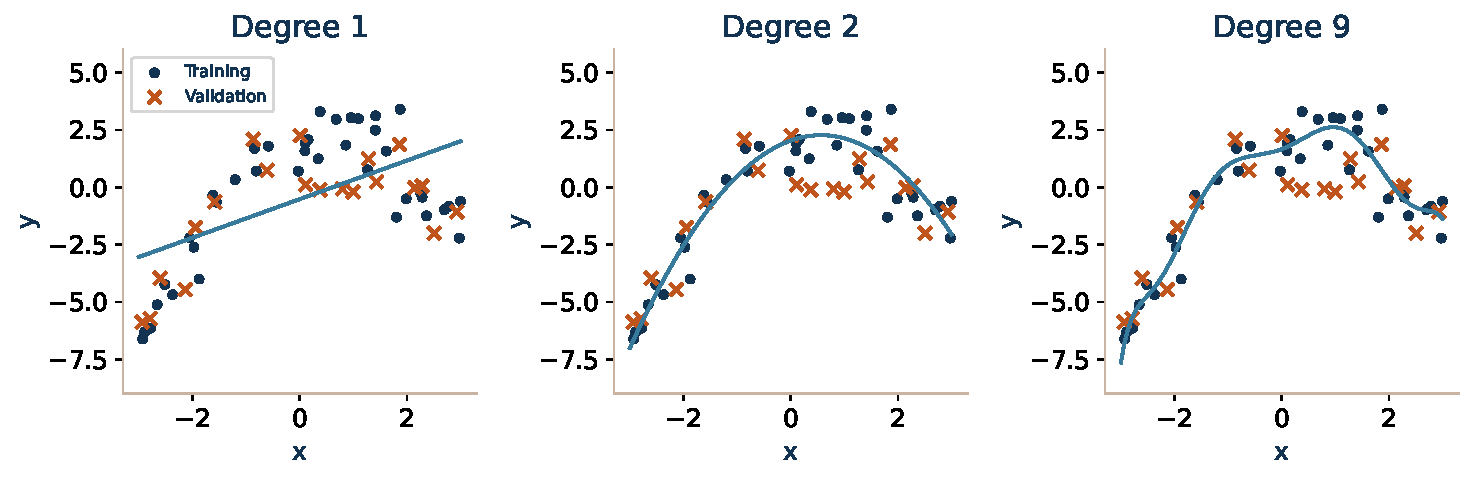
\includegraphics[width=.86\textwidth,height=.64\textheight,keepaspectratio]{figures/supervised/complexity.pdf}\par\small Same fictional dataset and fixed split. Training fit improves with flexibility; validation fit need not.
\end{frame}

\begin{frame}{Training and validation error}
\begin{center}\begin{tabular}{lrr}\toprule
Polynomial degree & Training RMSE & Validation RMSE\\\midrule 1 & 2.316 & 1.920\\ 2 & 0.931 & 1.288\\ 9 & 0.847 & 1.328\\
\bottomrule\end{tabular}\end{center}\begin{itemize}
\item The quadratic has the smallest validation RMSE among these candidates.
\item This comparison uses validation data; it is not a final test result.
\item With a small validation set, differences can be unstable.
\end{itemize}
\end{frame}

\begin{frame}{Bias and variance}
\begin{itemize}
\item A rigid model can miss systematic structure: underfitting.
\item A highly flexible model can react strongly to sampling noise: overfitting.
\item More training data, appropriate regularisation and validation can help.
\item For squared-error prediction, expected test error decomposes into squared bias, variance and irreducible noise under the usual model.
\end{itemize}
\end{frame}

\begin{frame}{Cross-validation}
\begin{itemize}
\item Divide the development data into $K$ folds.
\item Fit on $K-1$ folds and predict the held-out fold.
\item Repeat until every development observation has a held-out prediction.
\item Compare candidate procedures using the pooled out-of-fold loss.
\item Refit the chosen procedure on development data; evaluate on untouched test data.
\end{itemize}All preprocessing and feature selection belong inside each training fold.
\end{frame}

\begin{frame}{Linear regression as a learning method}
\[\hat y=\hat\beta_0+\hat\beta_1x_1+\cdots+\hat\beta_px_p\]\begin{itemize}
\item Estimates a conditional mean using a linear combination of features.
\item Uses squared-error minimisation.
\item Can include indicators, interactions and transformed predictors.
\item An interpretable baseline for more flexible prediction methods.
\end{itemize}
\end{frame}

\begin{frame}{Logistic regression as a learning method}
\[\hat p=\frac{1}{1+e^{-\hat\eta}},\qquad\hat\eta=\hat\beta_0+\sum_{j=1}^p\hat\beta_jx_j\]\begin{itemize}
\item Models the probability of a binary outcome.
\item Produces probabilities between 0 and 1.
\item A threshold turns a probability into a class decision.
\item Evaluate probabilities and class decisions separately.
\end{itemize}
\end{frame}

\begin{frame}{Other supervised methods}
\begin{center}\begin{tabular}{lp{.65\textwidth}}\toprule
Method & Main idea\\\midrule Nearest neighbours & Predict using similar training observations.\\ Decision trees & Split the predictor space into regions.\\ Random forests & Average many randomised trees.\\ Boosting & Combine successive models that improve the loss.\\ Neural networks & Learn compositions of nonlinear transformations.\\
\bottomrule\end{tabular}\end{center}The same split discipline and evaluation principles apply to every method.
\end{frame}

\begin{frame}{Human-centred evaluation}
\begin{itemize}
\item What outcome is actually recorded, and whose outcomes are missing?
\item Which false positives and false negatives matter to the people affected?
\item Are probabilities calibrated in the population where they will be used?
\item How will users understand, question and correct a prediction?
\item Monitor errors and changes in the data after deployment.
\end{itemize}
\end{frame}

\begin{frame}{E-tivity and R laboratory}
\begin{itemize}
\item E-tivity: define a task, detect leakage and explore model complexity.
\item Compare training and validation errors using a fixed small dataset.
\item R laboratory: \texttt{04\_validation\_and\_cv.R}.
\item Optional extension: compare logistic regression and a shallow tree.
\item Submit a short justification of the target, split and evaluation metric.
\end{itemize}
\end{frame}

\begin{frame}{Checkpoint}
\prompt{A model has excellent training accuracy but poor performance on later records. Give three possible explanations and one useful check for each.}\begin{itemize}
\item Possible explanations include overfitting, leakage and distribution change.
\item A test score evaluates the entire procedure under a particular sampling scheme.
\item Prediction quality, uncertainty and decision consequences must be considered together.
\end{itemize}
\end{frame}
